\documentclass{article}
\title{CSCI 2200 HW1}
\author{Xinshi,Wang}
\usepackage[letterpaper,textwidth=5.5in,right=0.6in,textheight=9in,left=0.6in,top=0.7in,bottom=0.7in]{geometry}
\usepackage{scrextend}
\usepackage{graphicx}
\usepackage{xcolor}
\usepackage{amssymb}
\usepackage{amsmath}
\usepackage{setspace}
\usepackage{mathrsfs}
\usepackage[utf8]{inputenc}
\usepackage{mathtools}
\begin{document}
\noindent
CSCI 2200 HW3\\
Wang Xinshi\\

%Q 13.10 starts from here
\begin{addmargin}[2em]{2em}
\text{\bf Problem 19.20.} A keychain has 10 similar keys. You are fumbling in the dark trying each key in a random order to
open your appartment door . What is the expected number of keys you try before you unlock the door? \\\\
Let x denote the number of trials before you unlock the door. Then we have $E[X] =  \sum_{x \in \omega} xP(x) = 0 \times \dfrac{1}{10} + 1 \times \dfrac{1}{10} + 2 \times \dfrac{1}{10} + ... + 10 \times \dfrac{1}{10} = \dfrac{1}{10} \times \sum_{i=0}{10} i = 5.5$
\end{addmargin}
%Q 13.10 ends here 

\clearpage

%Q 13.51 starts from here
\begin{addmargin}[2em]{2em}
	\text{\bf Problem 19.21.} You randomly guess every answer on a multiple choice exam with 50 questions and 4 possible
	answers per question. What is the expected number of questions you answer correctly?\\\\
	Let x denote the number of expected questions you answer correctly. Then we have $E[X] = np = \dfrac{1}{4} \times 50 = 12.5.$
\end{addmargin}
%Q 11.13 ends here
\clearpage


\begin{addmargin}[2em]{2em}
	\text{\bf Problem 19.38.} A box has 1024 fair and 1 two-headed coin. You pick a coin randomly, make 10 flips and get all H.\\
	(a) You flip the same coin you picked 100 times. What is the expected number of H?\\\\
	Let $X$ denote the expected number of H, we have $E[X] = P(fair)E[X|fair]+P(two-headed)E[X|two-headed] = \dfrac{9}{10}\times \dfrac{100+1}{2} + \dfrac{1}{10} \times 100  = 55.45$\\\\
	(b) You flip the same coin you picked unitl you get H. What is the expected number of flips you make?\\\\
		Let $X$ denote the expected number of trails to get an H, we have $E[X] = P(fair)E[X|fair]+P(two-headed)E[X|two-headed] = \dfrac{9}{10} \times 2 + \dfrac{1}{10} \times 0  = \dfrac{18}{10} = 1.8$\\\\
\end{addmargin}

%Q 12.74(k) ends here
\clearpage

\begin{addmargin}[2em]{2em}
	\text{\bf Problem 20.11.} Ten sailors return from shore and sleep randomly in their ten bunks (one sailor per bunk).\\
	(a) Let X be the number of sailors in the correct bunk. Compute (i) P[X = 10] (ii) P[X = 9] (iii) P[X = 8].\\
	(b) Compute the expected number of sailors in the correct bunk, that is E[X].\\\\
	(a). \\(i).$P[X = 10] = \dfrac{1}{10!} = \dfrac{1}{3628800} = 2.755 \times 10^{-7}$\\
	(ii) $P[X = 9] = 0$ Only one person sleeping on the wrong bed is impossible\\
	(iii) $P[X = 8] = \dfrac{1}{8!} \sum_{i=0}^{2} \dfrac{(-1)^i}{i!} =  1.24 \times 10^{-5}$\\\\
	(b). \\
	$E[X] = \sum_{x \in \omega} xP(x) = 2 \times \dfrac{P_{10}^5}{10!}+...+10 \times \dfrac{P_{10}^0}{10!}$(add them up when the remainder of i divides 2 is 0). we calculate using the following code\\
	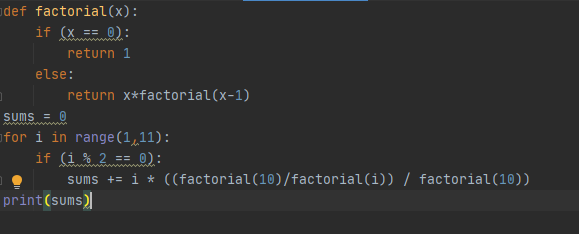
\includegraphics{"C:/Users/Micha/OneDrive - Rensselaer Polytechnic Institute/CSCI 2200/Latex_pictures/code.png"}\\
	which gives us 1.175.
\end{addmargin}
\clearpage
\begin{addmargin}[2em]{2em}
	\text{\bf Problem 20.23.} Five students independently get a random number in {1, . . . , 10}. A score is increased for every
	pair of student whose numbers agree. Find the expected score when:\\
	(a) For every pair of students whose numbers agree, the score is increased by 1.\\
	 Since after one person chooses, there are only four people left, and the probability of forming a pair with the one person is $\dfrac{1}{10}$ for all the four students. Let $X$ denote the expected score, and thus we have 
	 $$E[X] = \dfrac{5 \times 4 \times \dfrac{1}{10}}{2} = 1$$
	(b) For every pair of students whose numbers agree, the score is increased by the number the pair has.\\
		On average(the expected value), every pair has a number of $1 \times \dfrac{1}{10} + 2 \times \dfrac{1}{10} + ... + 10 \times \dfrac{1}{10} = 5.5 $ Thus $$E[X] = \dfrac{5.5 \times 5 \times 4 \times \dfrac{1}{10}}{2} = 5.5$$ \\
	(c) Generalize (a) and (b) to n students independently getting a number in {1, . . . , k}.\\
		$$E[X] = \dfrac{\dfrac{n+1}{2} \times n \times (n-1) \times \dfrac{1}{k}}{2}$$
\end{addmargin}
\clearpage
\begin{addmargin}[2em]{2em}
	\text{\bf Problem 20.20(j ).}20 kids stand in line. A random pair of adjacent standing kids pair up and sit. This continues until no more pairs
	can be formed. What is the expected number of unpaired kids?\\
	Let $S(n)$ denote the number of students standing. For $20$ people, we have $S(20) = \dfrac{1}{19} S(0) + S(18) + \dfrac{1}{19} S(1) + S(17) + \dfrac{1}{19} S(18) + S(0)$. With base case $n = 1$ and $3$ return $1$ and $n = 0$ and $2$ return $0$. According to python, we have $S(20) = 2.977$.
\end{addmargin}
\end{document}